\documentclass{standalone}
\usepackage{tikz}
\usetikzlibrary{patterns, positioning}


\begin{document}
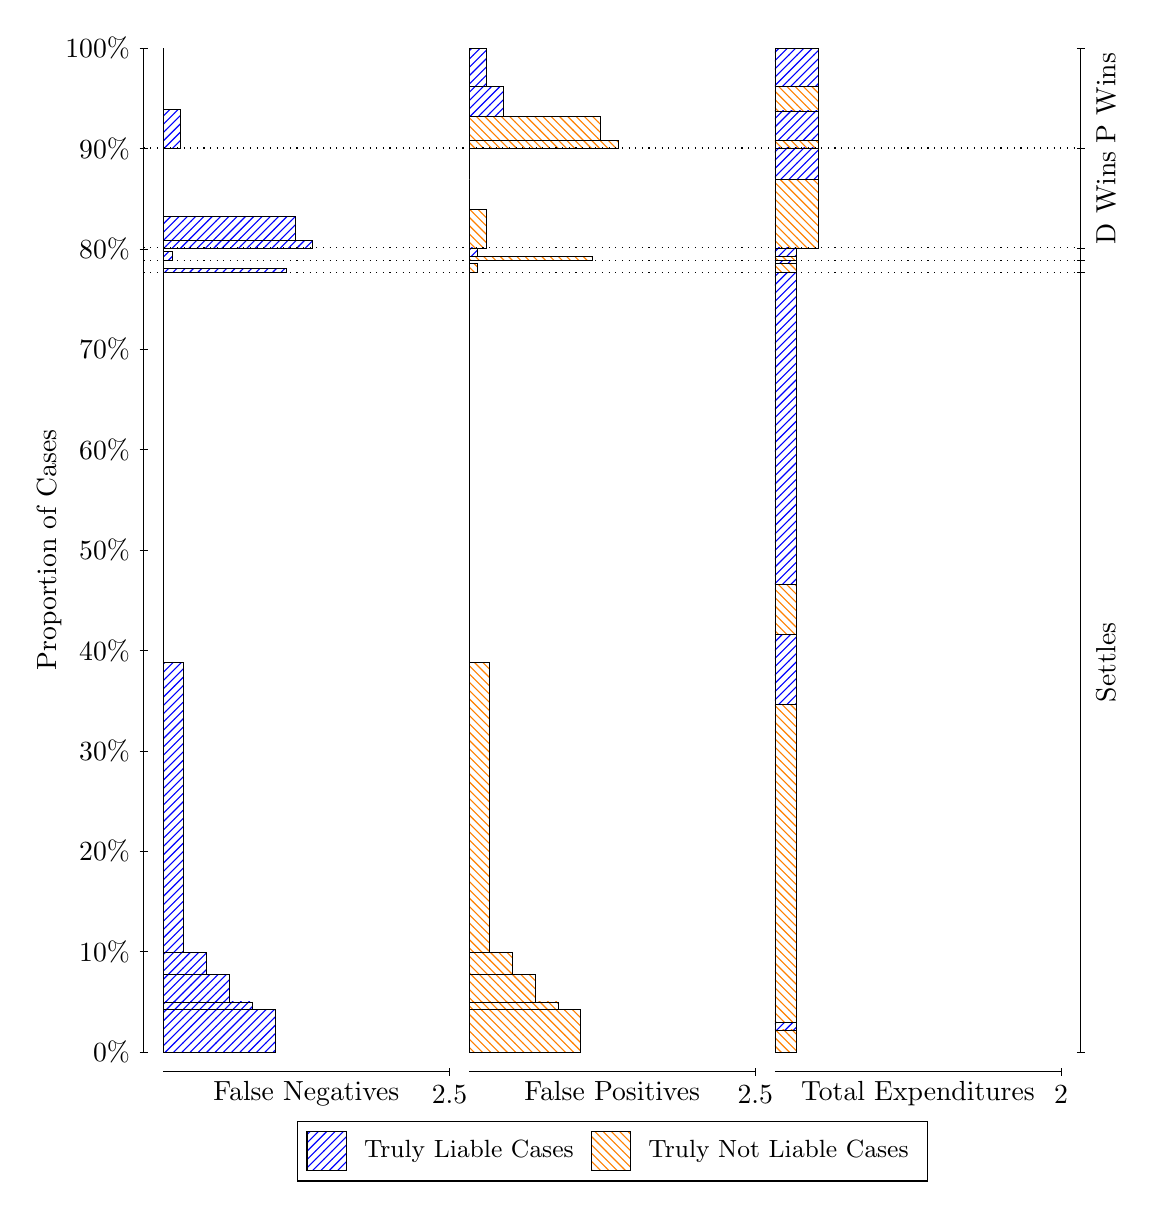
\begin{tikzpicture}
\draw[black, very thin] (1.5,1.75) -- (1.5,14.5);
\node[rotate=90, text=black, anchor=center] at (0.3, 8.125) {Proportion of Cases};
\draw[black, very thin] (1.45,1.75) -- (1.55,1.75);
\node[text=black, anchor=east] at (1.45, 1.75) {0\%};
\draw[black, very thin] (1.45,3.025) -- (1.55,3.025);
\node[text=black, anchor=east] at (1.45, 3.025) {10\%};
\draw[black, very thin] (1.45,4.3) -- (1.55,4.3);
\node[text=black, anchor=east] at (1.45, 4.3) {20\%};
\draw[black, very thin] (1.45,5.575) -- (1.55,5.575);
\node[text=black, anchor=east] at (1.45, 5.575) {30\%};
\draw[black, very thin] (1.45,6.85) -- (1.55,6.85);
\node[text=black, anchor=east] at (1.45, 6.85) {40\%};
\draw[black, very thin] (1.45,8.125) -- (1.55,8.125);
\node[text=black, anchor=east] at (1.45, 8.125) {50\%};
\draw[black, very thin] (1.45,9.4) -- (1.55,9.4);
\node[text=black, anchor=east] at (1.45, 9.4) {60\%};
\draw[black, very thin] (1.45,10.675) -- (1.55,10.675);
\node[text=black, anchor=east] at (1.45, 10.675) {70\%};
\draw[black, very thin] (1.45,11.95) -- (1.55,11.95);
\node[text=black, anchor=east] at (1.45, 11.95) {80\%};
\draw[black, very thin] (1.45,13.225) -- (1.55,13.225);
\node[text=black, anchor=east] at (1.45, 13.225) {90\%};
\draw[black, very thin] (1.45,14.5) -- (1.55,14.5);
\node[text=black, anchor=east] at (1.45, 14.5) {100\%};

\draw[black, very thin] (13.4,1.75) -- (13.4,14.5);
\draw[black, very thin] (13.35,1.75) -- (13.45,1.75);
\node[anchor=west] at (13.35, 1.75) {};
\draw[black, very thin] (13.35,11.651) -- (13.45,11.651);
\node[anchor=west] at (13.35, 11.651) {};
\draw[black, very thin] (13.35,11.807) -- (13.45,11.807);
\node[anchor=west] at (13.35, 11.807) {};
\draw[black, very thin] (13.35,11.963) -- (13.45,11.963);
\node[anchor=west] at (13.35, 11.963) {};
\draw[black, very thin] (13.35,13.231) -- (13.45,13.231);
\node[anchor=west] at (13.35, 13.231) {};
\draw[black, very thin] (13.35,14.5) -- (13.45,14.5);
\node[anchor=west] at (13.35, 14.5) {};

\draw[black, very thin, pattern color=blue, pattern=north east lines] (1.75,1.75) rectangle (3.167,2.2871);
\draw[black, very thin, pattern color=blue, pattern=north east lines] (1.75,2.2871) rectangle (2.8763,2.3852);
\draw[black, very thin, pattern color=blue, pattern=north east lines] (1.75,2.3852) rectangle (2.5857,2.734);
\draw[black, very thin, pattern color=blue, pattern=north east lines] (1.75,2.734) rectangle (2.295,3.014);
\draw[black, very thin, pattern color=blue, pattern=north east lines] (1.75,3.014) rectangle (2.0043,6.7006);
\draw[black, very thin, pattern color=orange, pattern=north west lines] (1.75,6.7006) rectangle (1.75,11.651);
\draw[black, very thin, pattern color=blue, pattern=north east lines] (1.75,11.651) rectangle (3.3123,11.697);
\draw[black, very thin, pattern color=orange, pattern=north west lines] (1.75,11.697) rectangle (1.75,11.807);
\draw[black, very thin, pattern color=blue, pattern=north east lines] (1.75,11.807) rectangle (1.859,11.917);
\draw[black, very thin, pattern color=orange, pattern=north west lines] (1.75,11.917) rectangle (1.75,11.963);
\draw[black, very thin, pattern color=blue, pattern=north east lines] (1.75,11.963) rectangle (3.6393,12.055);
\draw[black, very thin, pattern color=blue, pattern=north east lines] (1.75,12.055) rectangle (3.4213,12.361);
\draw[black, very thin, pattern color=orange, pattern=north west lines] (1.75,12.361) rectangle (1.75,13.231);
\draw[black, very thin, pattern color=blue, pattern=north east lines] (1.75,13.231) rectangle (1.968,13.723);
\draw[black, very thin, pattern color=orange, pattern=north west lines] (1.75,13.723) rectangle (1.75,14.121);
\draw[black, very thin, pattern color=blue, pattern=north east lines] (1.75,14.121) rectangle (1.75,14.5);
\draw[black, very thin, pattern color=orange, pattern=north west lines] (5.6333,1.75) rectangle (7.0503,2.287);
\draw[black, very thin, pattern color=orange, pattern=north west lines] (5.6333,2.287) rectangle (6.7597,2.3852);
\draw[black, very thin, pattern color=orange, pattern=north west lines] (5.6333,2.3852) rectangle (6.469,2.734);
\draw[black, very thin, pattern color=orange, pattern=north west lines] (5.6333,2.734) rectangle (6.1783,3.014);
\draw[black, very thin, pattern color=orange, pattern=north west lines] (5.6333,3.014) rectangle (5.8877,6.7007);
\draw[black, very thin, pattern color=blue, pattern=north east lines] (5.6333,6.7007) rectangle (5.6333,11.651);
\draw[black, very thin, pattern color=orange, pattern=north west lines] (5.6333,11.651) rectangle (5.7423,11.762);
\draw[black, very thin, pattern color=blue, pattern=north east lines] (5.6333,11.762) rectangle (5.6333,11.807);
\draw[black, very thin, pattern color=orange, pattern=north west lines] (5.6333,11.807) rectangle (7.1957,11.852);
\draw[black, very thin, pattern color=blue, pattern=north east lines] (5.6333,11.852) rectangle (5.7423,11.963);
\draw[black, very thin, pattern color=orange, pattern=north west lines] (5.6333,11.963) rectangle (5.8513,12.454);
\draw[black, very thin, pattern color=orange, pattern=north west lines] (5.6333,12.454) rectangle (5.6333,12.832);
\draw[black, very thin, pattern color=blue, pattern=north east lines] (5.6333,12.832) rectangle (5.6333,13.231);
\draw[black, very thin, pattern color=orange, pattern=north west lines] (5.6333,13.231) rectangle (7.5227,13.324);
\draw[black, very thin, pattern color=orange, pattern=north west lines] (5.6333,13.324) rectangle (7.3047,13.63);
\draw[black, very thin, pattern color=blue, pattern=north east lines] (5.6333,13.63) rectangle (6.0693,14.009);
\draw[black, very thin, pattern color=blue, pattern=north east lines] (5.6333,14.009) rectangle (5.8513,14.5);
\draw[black, very thin, pattern color=orange, pattern=north west lines] (9.5167,1.75) rectangle (9.7892,2.03);
\draw[black, very thin, pattern color=blue, pattern=north east lines] (9.5167,2.03) rectangle (9.7892,2.1281);
\draw[black, very thin, pattern color=orange, pattern=north west lines] (9.5167,2.1281) rectangle (9.7892,6.1637);
\draw[black, very thin, pattern color=blue, pattern=north east lines] (9.5167,6.1637) rectangle (9.7892,7.0495);
\draw[black, very thin, pattern color=orange, pattern=north west lines] (9.5167,7.0495) rectangle (9.7892,7.6848);
\draw[black, very thin, pattern color=blue, pattern=north east lines] (9.5167,7.6848) rectangle (9.7892,11.651);
\draw[black, very thin, pattern color=orange, pattern=north west lines] (9.5167,11.651) rectangle (9.7892,11.762);
\draw[black, very thin, pattern color=blue, pattern=north east lines] (9.5167,11.762) rectangle (9.7892,11.807);
\draw[black, very thin, pattern color=orange, pattern=north west lines] (9.5167,11.807) rectangle (9.7892,11.852);
\draw[black, very thin, pattern color=blue, pattern=north east lines] (9.5167,11.852) rectangle (9.7892,11.963);
\draw[black, very thin, pattern color=orange, pattern=north west lines] (9.5167,11.963) rectangle (10.062,12.832);
\draw[black, very thin, pattern color=blue, pattern=north east lines] (9.5167,12.832) rectangle (10.062,13.231);
\draw[black, very thin, pattern color=orange, pattern=north west lines] (9.5167,13.231) rectangle (10.062,13.324);
\draw[black, very thin, pattern color=blue, pattern=north east lines] (9.5167,13.324) rectangle (10.062,13.702);
\draw[black, very thin, pattern color=orange, pattern=north west lines] (9.5167,13.702) rectangle (10.062,14.009);
\draw[black, very thin, pattern color=blue, pattern=north east lines] (9.5167,14.009) rectangle (10.062,14.5);
\draw[black, dotted] (1.5,11.651) -- (13.4,11.651);
\draw[black, dotted] (1.5,11.807) -- (13.4,11.807);
\draw[black, dotted] (1.5,11.963) -- (13.4,11.963);
\draw[black, dotted] (1.5,13.231) -- (13.4,13.231);
\draw[black, very thin] (1.75,1.5) -- (5.3833,1.5);
\node[text=black, anchor=north] at (3.5667, 1.5) {False Negatives};
\draw[black, very thin] (5.3833,1.45) -- (5.3833,1.55);
\node[text=black, anchor=north] at (5.3833, 1.45) {2.5};

\draw[black, very thin] (5.6333,1.5) -- (9.2667,1.5);
\node[text=black, anchor=north] at (7.45, 1.5) {False Positives};
\draw[black, very thin] (9.2667,1.45) -- (9.2667,1.55);
\node[text=black, anchor=north] at (9.2667, 1.45) {2.5};

\draw[black, very thin] (9.5167,1.5) -- (13.15,1.5);
\node[text=black, anchor=north] at (11.333, 1.5) {Total Expenditures};
\draw[black, very thin] (13.15,1.45) -- (13.15,1.55);
\node[text=black, anchor=north] at (13.15, 1.45) {2};

\node[text=black, centered, rotate=90] at (13.72, 6.7007) {Settles};


\node[text=black, centered, rotate=90] at (13.72, 12.597) {D Wins};
\node[text=black, centered, rotate=90] at (13.72, 13.866) {P Wins};

\draw (7.449999999999999,1.5) node[draw=none] (baseCoordinate) {};
\begin{scope}[align=center]
        \matrix[scale=0.5, draw=black, below=0.5cm of baseCoordinate, nodes={draw}, column sep=0.1cm]{
            \node[rectangle, draw, minimum width=0.5cm, minimum height=0.5cm, pattern color=blue, pattern=north east lines] {}; &
            \node[draw=none, font=\small, text=black] (B) {Truly Liable Cases}; &
            \node[rectangle, draw, minimum width=0.5cm, minimum height=0.5cm, pattern color=orange, pattern=north west lines] {}; &
            \node[draw=none, font=\small, text=black] (B) {Truly Not Liable Cases}; \\
            };
\end{scope}

\end{tikzpicture}
\end{document}